
\documentclass[12pt]{article}
\usepackage{graphicx}
\usepackage{float}
\usepackage[margin=1in]{geometry}
\usepackage{caption}

\begin{document}

\title{Analysis on Decision Tree Construction for Multi-class Classification of a Car Evaluation Dataset}
\author{Anik Saha, ID: 2005001}
\maketitle
\newpage

\section{Introduction}

Decision Tree is an tree-structure for conditional step-by-step decision making about particular data from given attributes. Decision trees are widely used for binary or multi-class classification problems. To select which attribute to choose while splitting a node in the tree, we consider using two different evaluation metrics, namely, Information Gain and Gini Impurity. In addition, we introduce the flexibility of choosing either the best performing attribute or one random from the top three performers at each level.

\section{Problem Description}

The problem is to classify cars as one of the 4 possible values "unacc", "acc", "good", "vgood".\\

The attributes provided are as follows:
\begin{itemize}
    \item buying
    \item maint
    \item doors
    \item persons
    \item lugboot
    \item safety
\end{itemize}

\section{Methodology}

We first split the dataset into train and test set randomly as per the split ratio. Then we construct the decision tree from the train set and evaluate its performance on the test set.\\

The attribute selection strategies tested are as follows:
\begin{itemize}
    \item Always taking the best attribute
    \item Selecting one randomly from the top three attributes
\end{itemize}

The evaluation metrics tested are as follows:
\begin{itemize}
    \item Information Gain
    \item Gini Impurity
\end{itemize}

\newpage

\section{Results} 


% Accuracy Comparison
\subsection{Accuracy Comparison}
\begin{table}[h]
\centering
\begin{tabular}{|p{5cm}|c|c|}
\hline
& \multicolumn{2}{c|}{Average accuracy over 20 runs} \\
\hline
Attribute selection strategy & Information gain & Gini impurity \\
\hline
Always select the best attribute & 93.28 & 92.54 \\
\hline
Select one randomly from the top three attributes & 81.49 & 81.42 \\
\hline
\end{tabular}
\end{table}


% Combined Accuracy Distribution
\subsection{Overall Accuracy Distribution}
\begin{figure}[H]
    \centering
    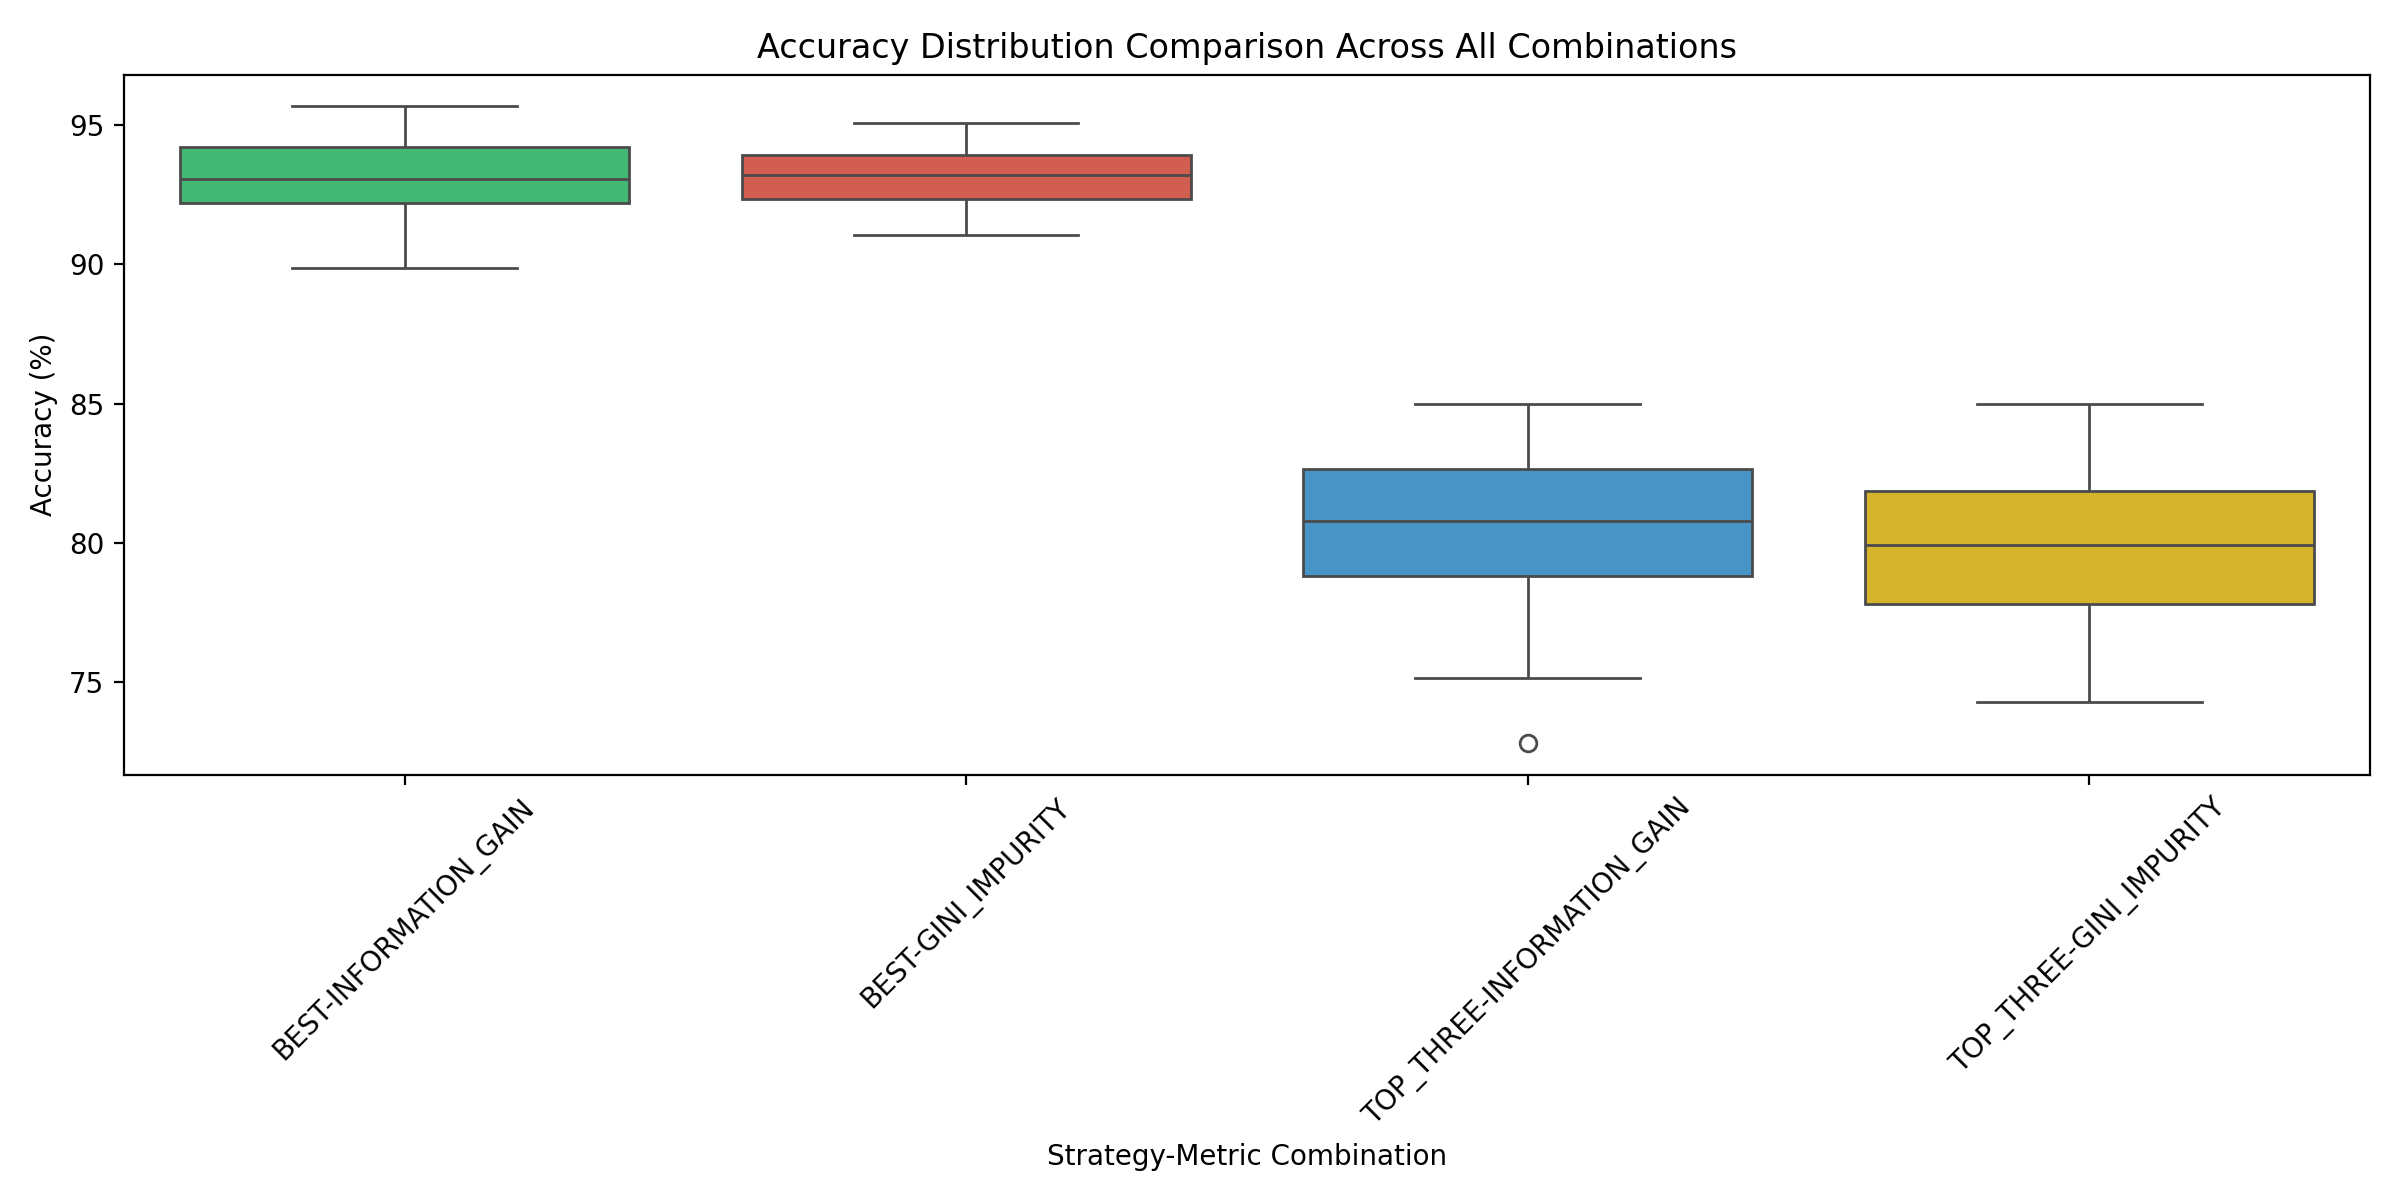
\includegraphics[width=0.9\textwidth]{plots/combined_accuracy_distribution.png}
    \caption{Comparison of accuracy distributions across different strategy and metric combinations.}
    \label{fig:combined-accuracy}
\end{figure}

The above box-whisker plot demonstrates the test-set accuracy of the decision tree built in case of 4 different combinations of selection strategy and evaluation metrics.

It is evident that the accuracy attains its maximum when we take the best attribute while testing at each node and the evaluation metric is set to be the Information Gain. The accuracy, in case of Gini Impurity is also very close to the previous case. However, when we pick one random attribute from the top three, not only does the mean accuracy drop, but also does the accuracy deviate more over several runs, thereby making it less consistent.

\newpage

% Combined Confusion Matrices
\subsection{Confusion Matrices}
\begin{figure}[H]
    \centering
    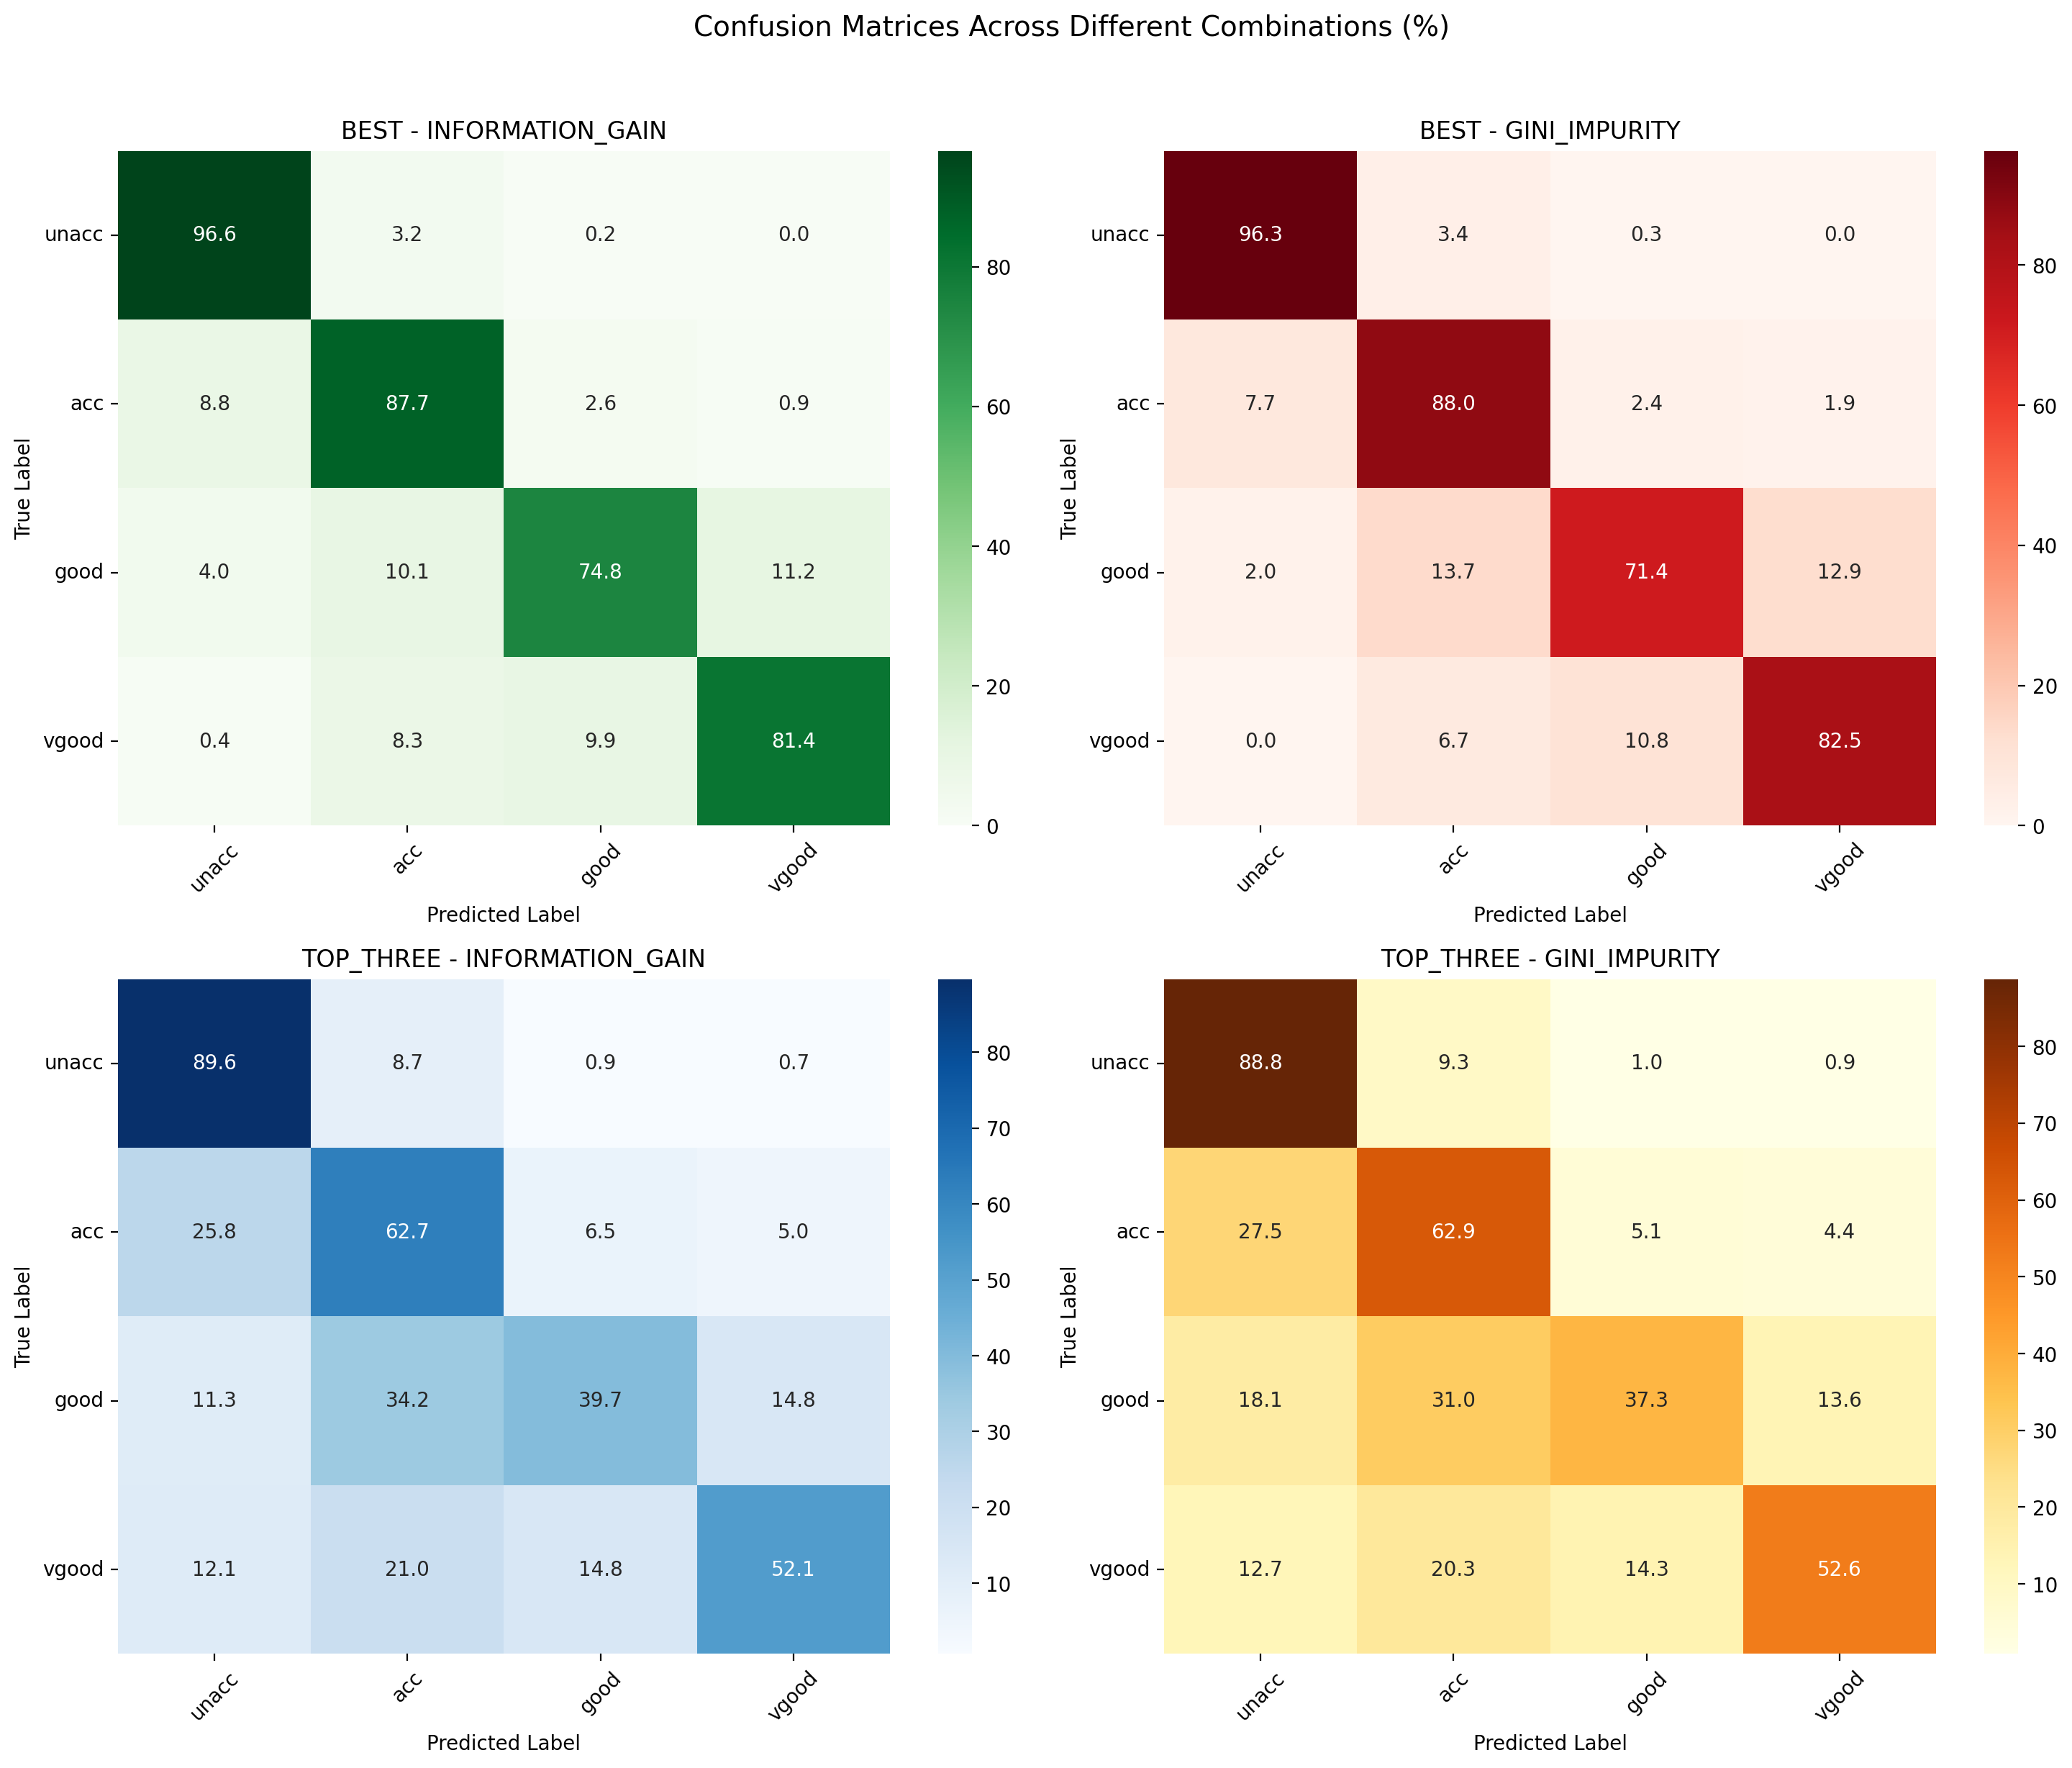
\includegraphics[width=\textwidth]{plots/confusion_matrices_combined.png}
    \caption{Confusion matrices showing classification performance across different strategy-metric combinations. Each subplot uses a different color gradient for better distinction.}
    \label{fig:confusion-matrices}
\end{figure}

The confusion matrices give insights about which class pairs the decision tree often confuse between.

For instance, it often classifies "good" ones as "acc", as can be observed in all of the confusion matrices. And in case of random-choice from three attributes, it also often tends to classify "vgood" classes as "acc" or "good". Also, in case of random picking from top three, the confusion matrix appears more scattered and inconsistencies are higher.

\newpage

% Combined Error Rates
\subsection{Error Rate Analysis}
\begin{figure}[H]
    \centering
    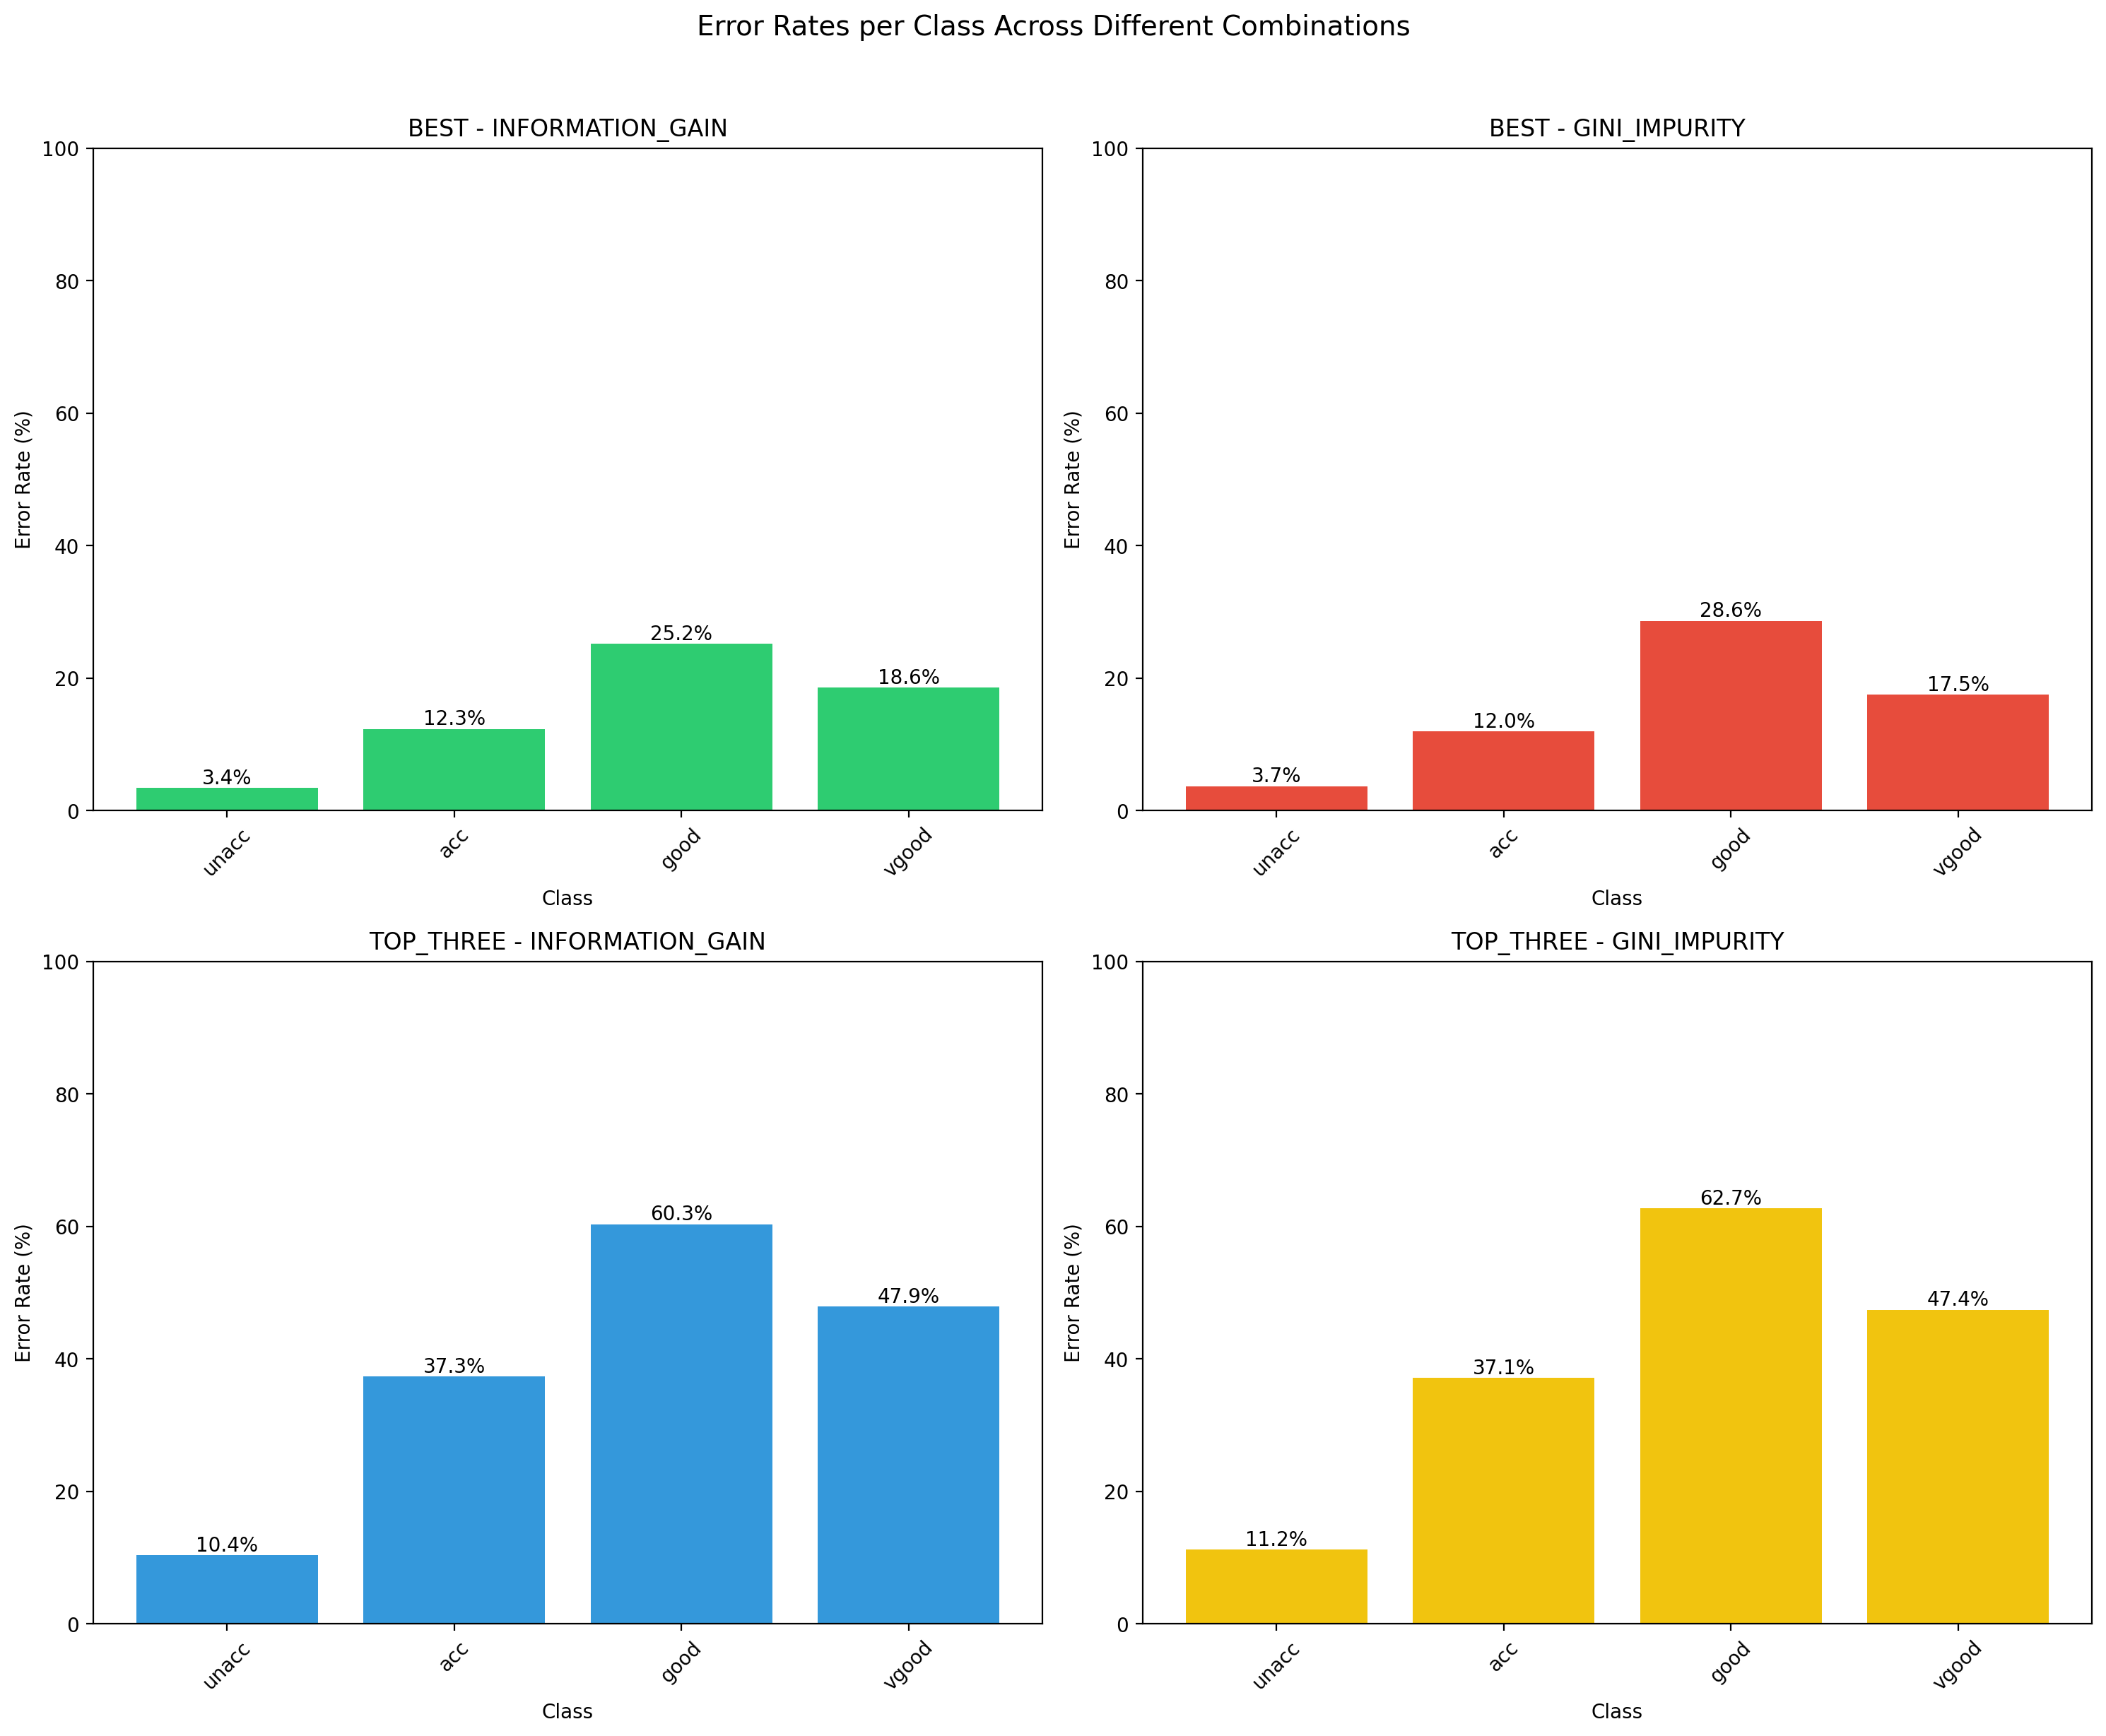
\includegraphics[width=\textwidth]{plots/error_rates_combined.png}
    \caption{Error rates per class across different strategy-metric combinations, showing the misclassification percentages for each category.}
    \label{fig:error-rates}
\end{figure}

These plots show that the decision tree, in almost all cases, classifies "unacc" classes correctly. On the contrary, the maximum error rates are observed in case of "good" class.

\newpage

% Attribute Depths (Individual plots still)
\subsection{Attribute Depth Analysis}
\begin{figure}[H]
    \centering
    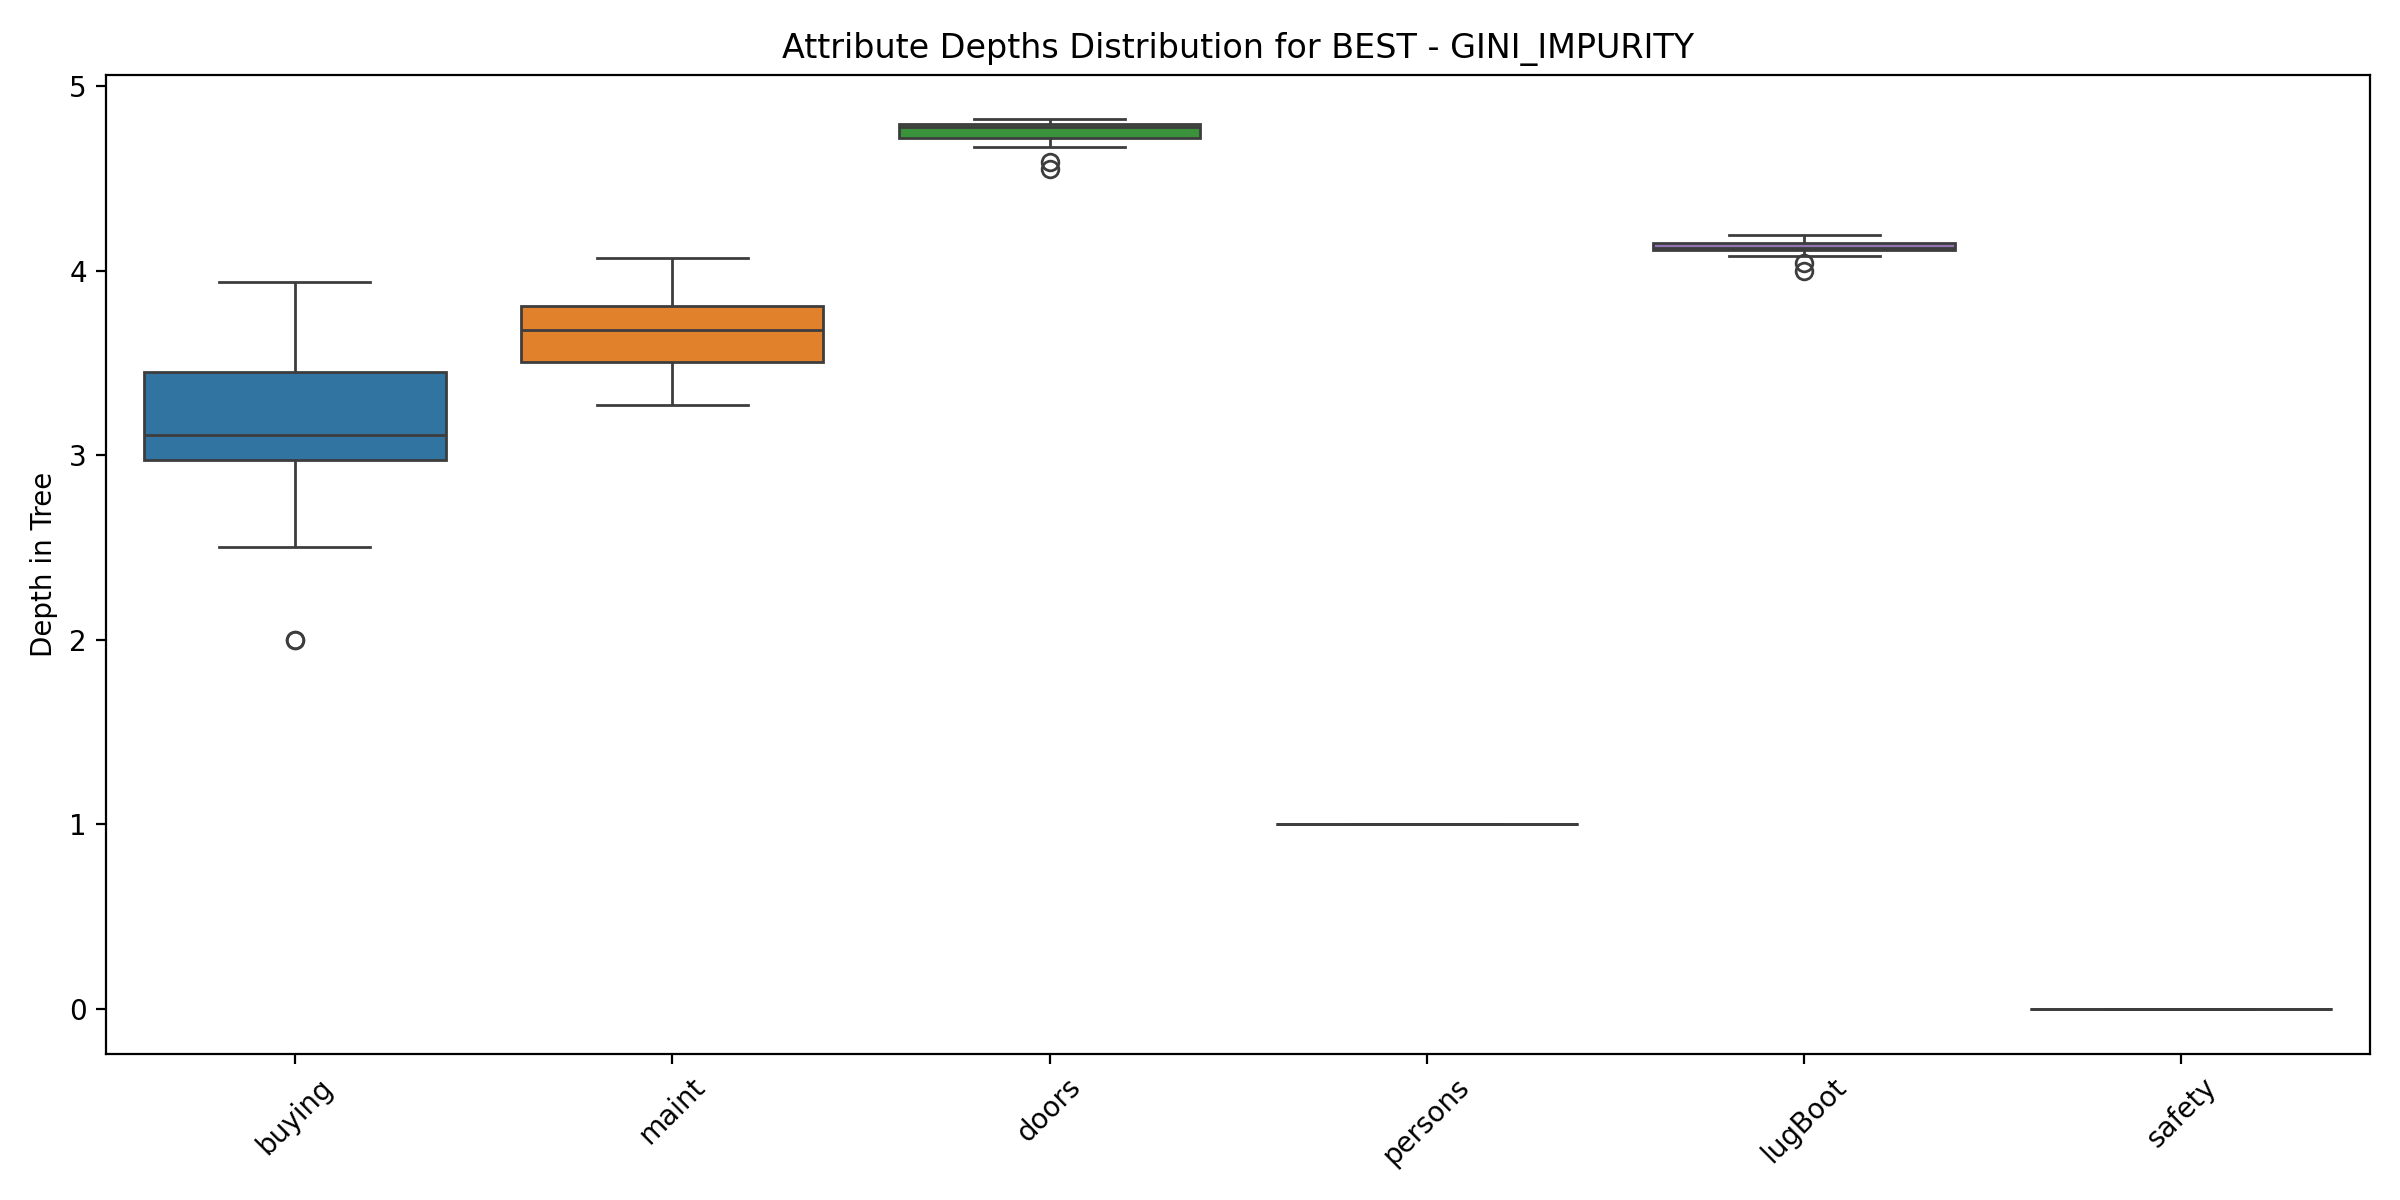
\includegraphics[width=0.9\textwidth]{plots/attribute_depths_BEST_GINI_IMPURITY.png}
    \caption{Distribution of attribute depths for BEST strategy with GINI IMPURITY metric.}
    \label{fig:attr-best-gini}
\end{figure}

This box whisker plot, shows an analysis of the attribute depths. An attribute with lower depth in the tree indicates that it is more crucial in the classification decision. Here, it can be seen that the attributes "safety" and "persons" are the most crucial having depths 0 and 1 consistently in the tree. This means they lie on the topmost decision nodes almost always. Others are placed at higher depths.

\newpage

\begin{figure}[H]
    \centering
    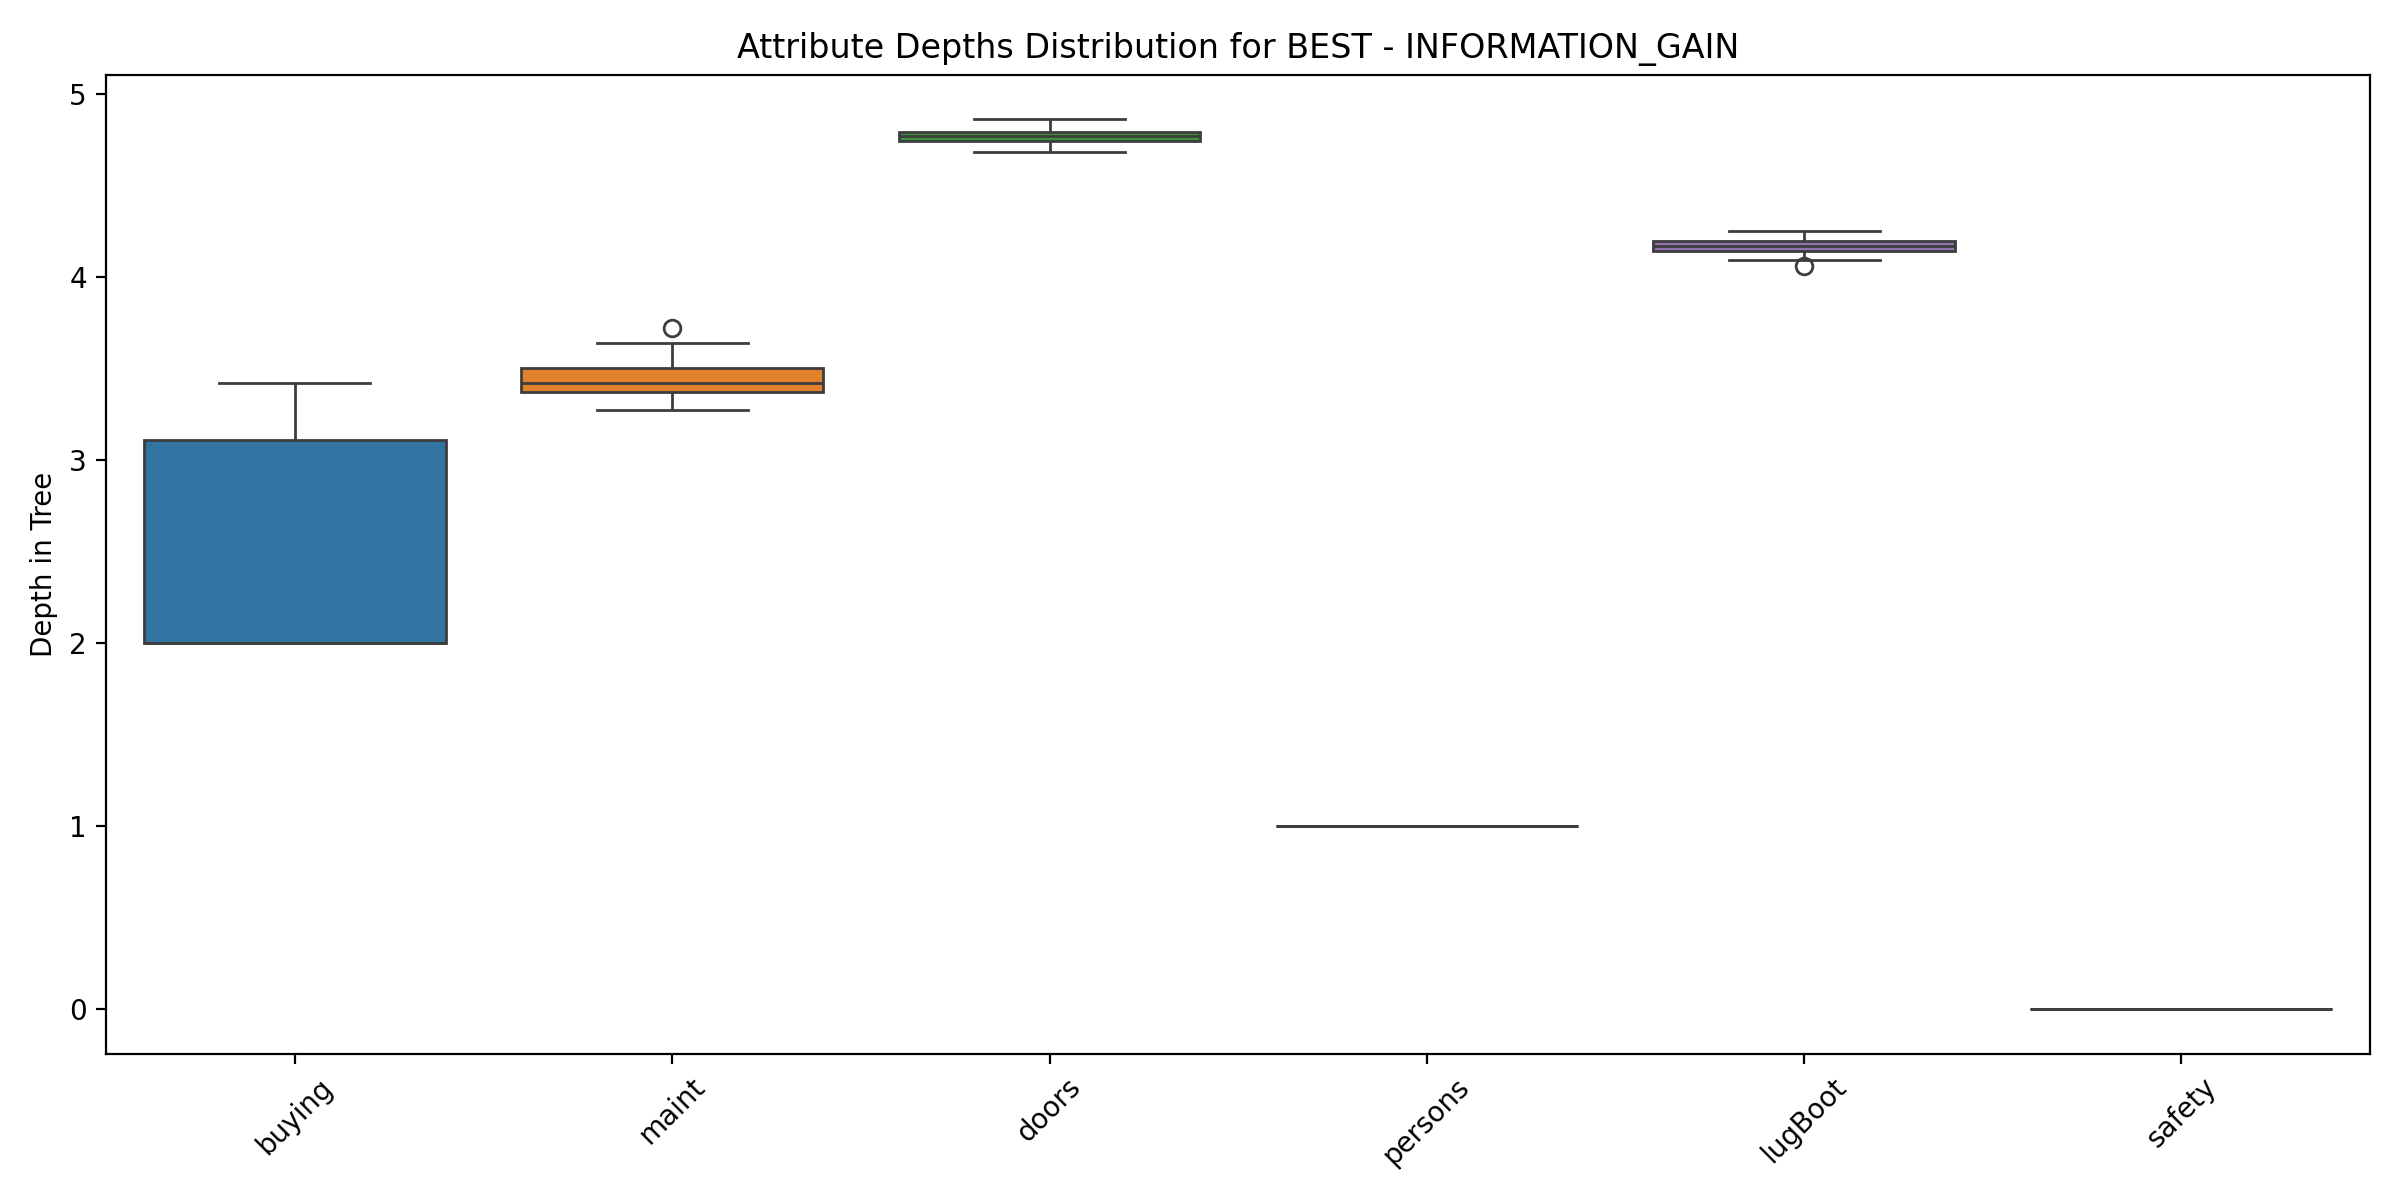
\includegraphics[width=0.9\textwidth]{plots/attribute_depths_BEST_INFORMATION_GAIN.png}
    \caption{Distribution of attribute depths for BEST strategy with INFORMATION GAIN metric.}
    \label{fig:attr-best-ig}
\end{figure}

This plot for the case of Information Gain is very similar to the one above.

\newpage

\begin{figure}[H]
    \centering
    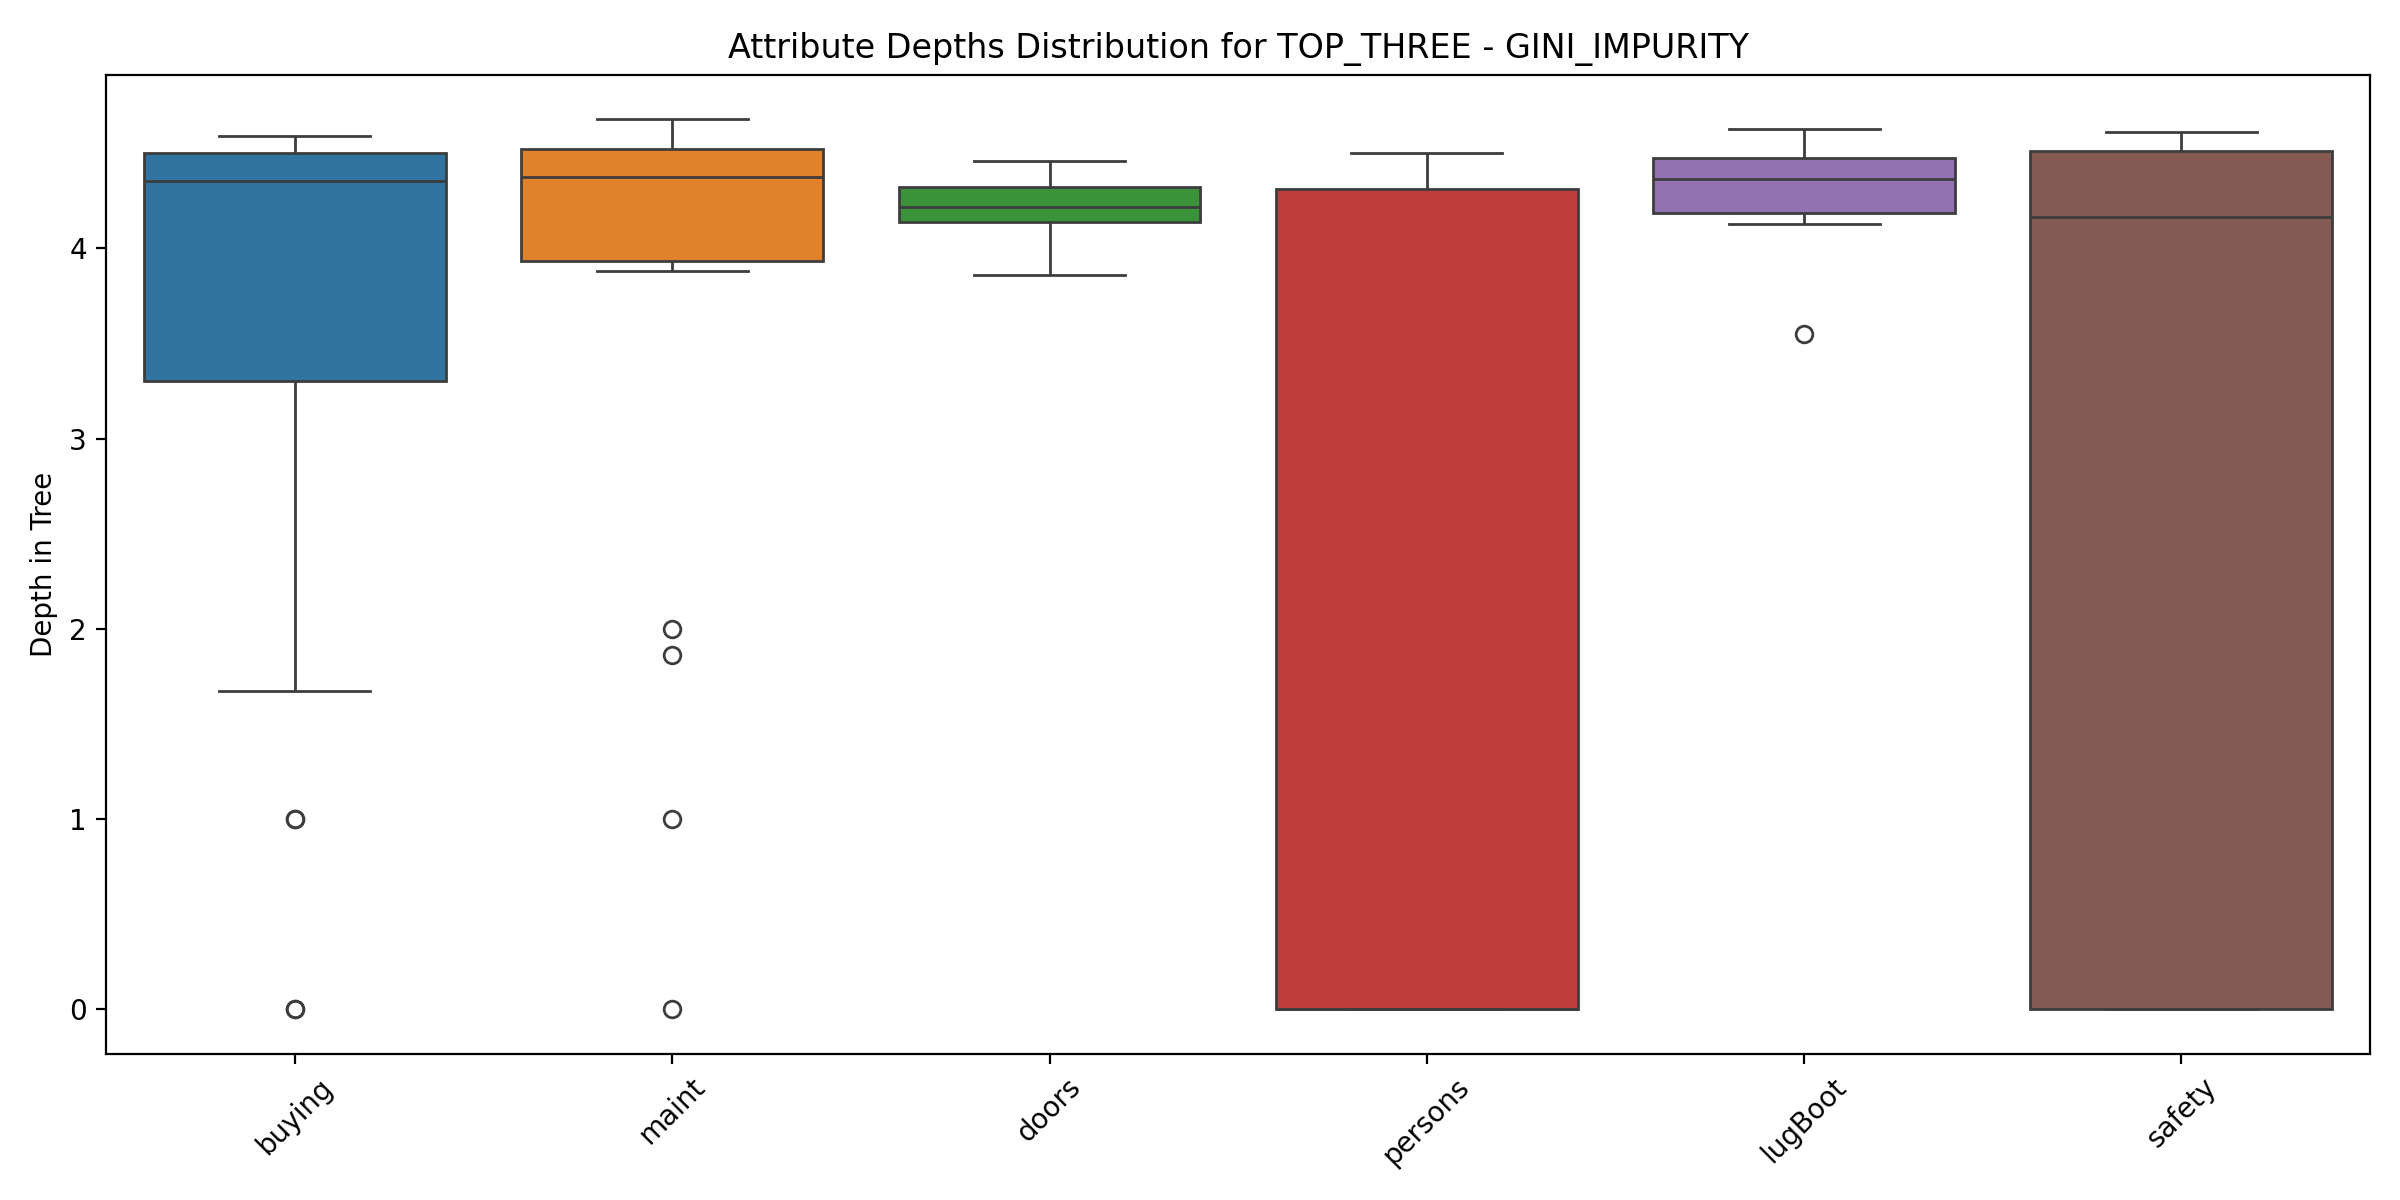
\includegraphics[width=0.9\textwidth]{plots/attribute_depths_TOP_THREE_GINI_IMPURITY.png}
    \caption{Distribution of attribute depths for TOP THREE strategy with GINI IMPURITY metric.}
    \label{fig:attr-top3-gini}
\end{figure}

When we switch the selection strategy, these plots change drastically. The attributes "persons" and "safety" which were always placed closer to the root in the above cases, are now rather being placed at scattered depths ranging from 0 to 5. The reason is that, at the first nodes, due to random choices, often the optimal ones are rejected. And later, they are being placed at scattered positions in the tree. This also explains why the overall accuracy drops significantly in case of random choice.

\newpage

\begin{figure}[H]
    \centering
    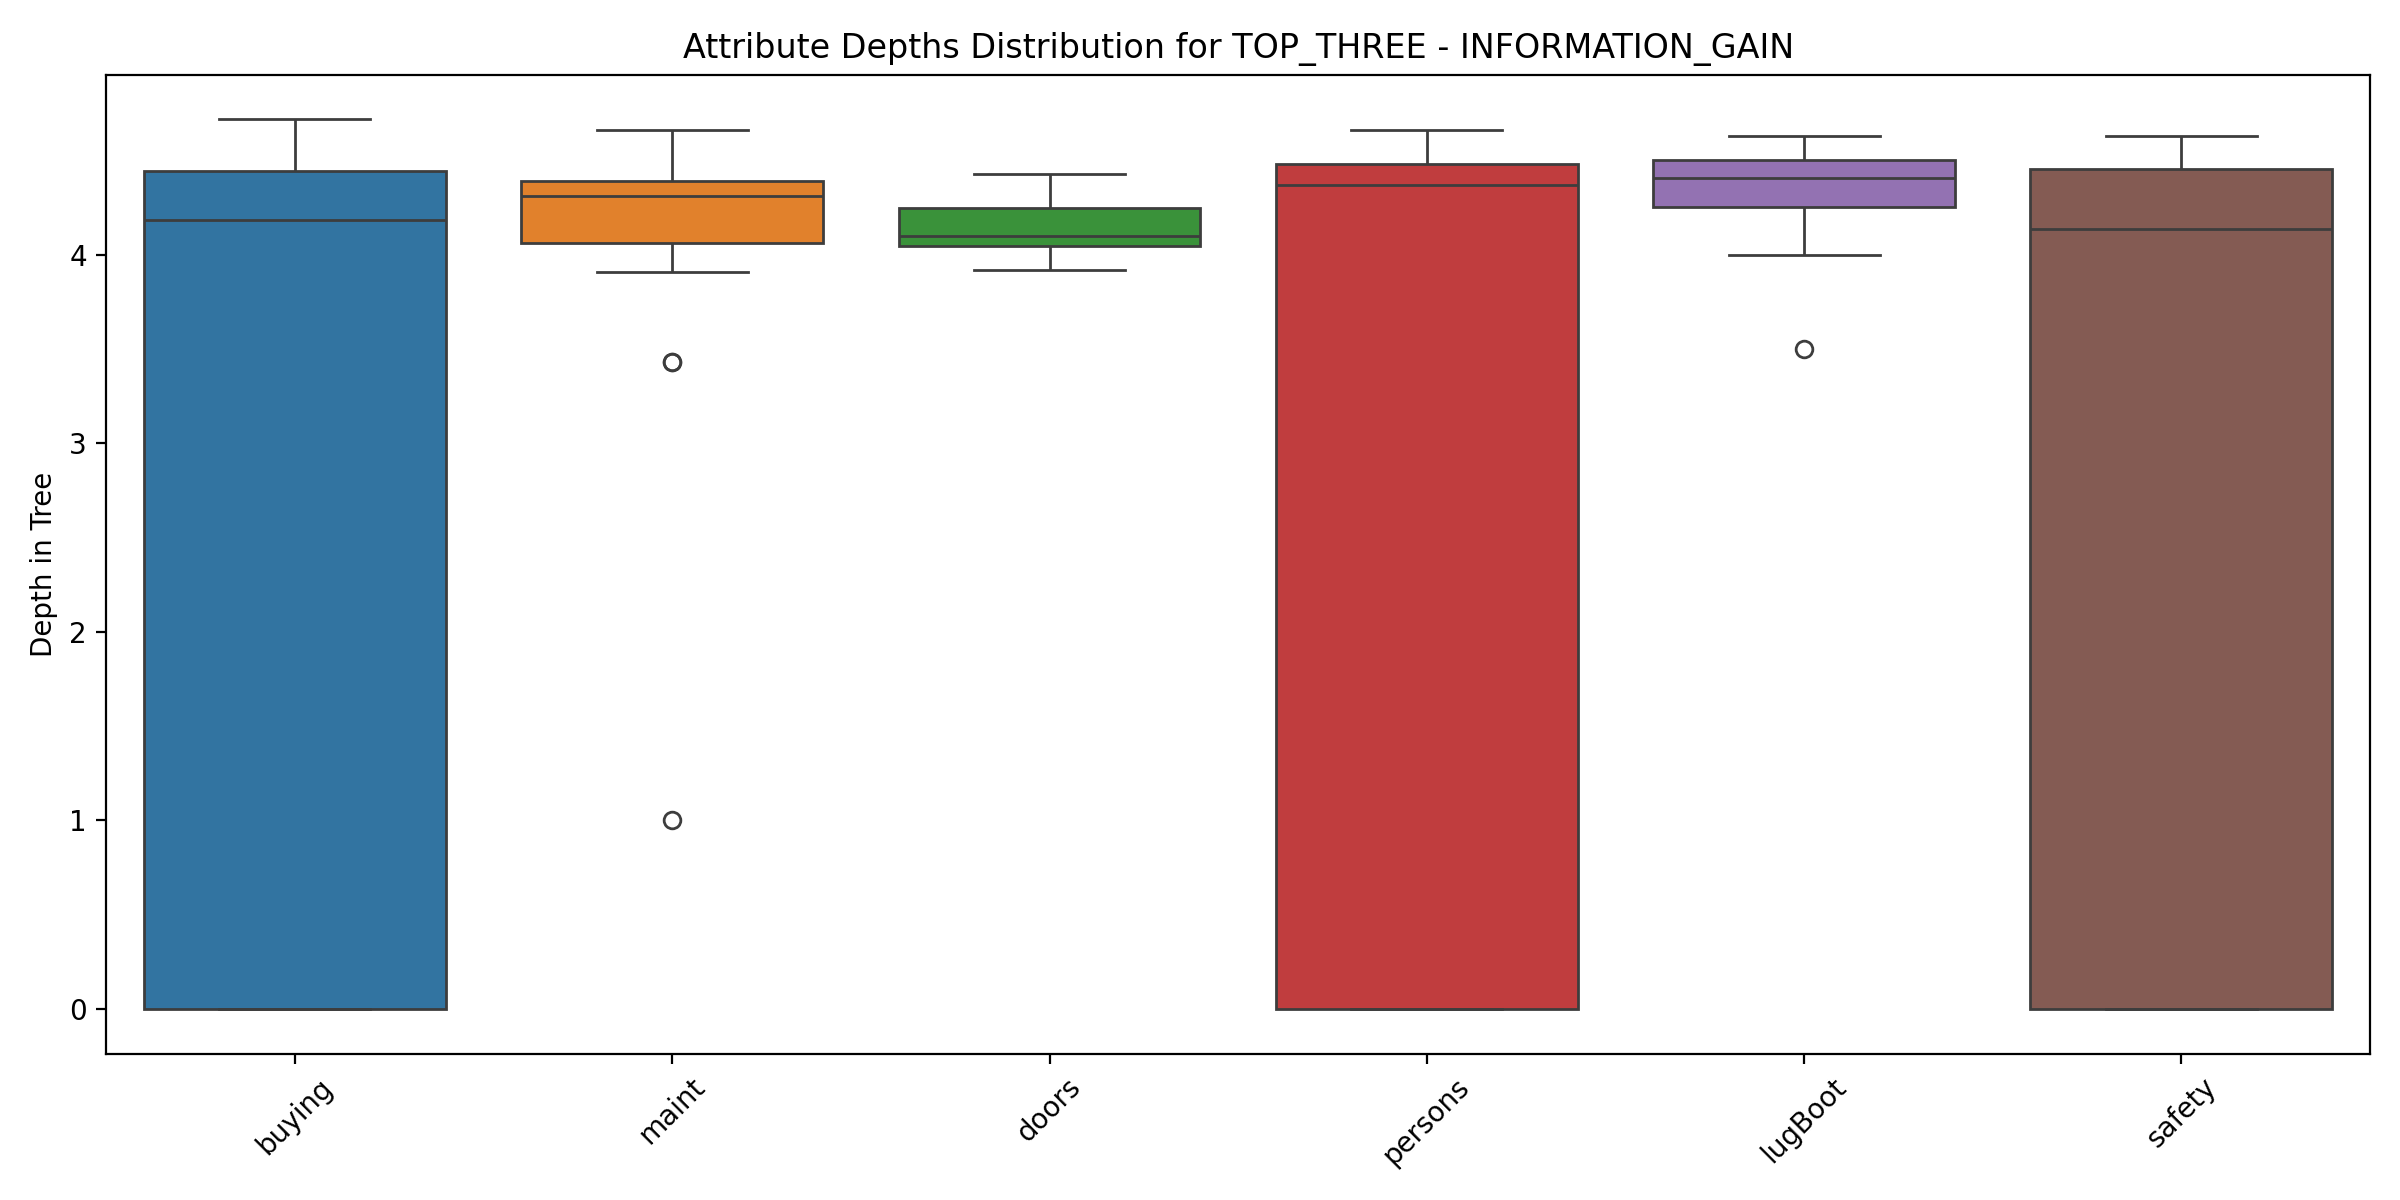
\includegraphics[width=0.9\textwidth]{plots/attribute_depths_TOP_THREE_INFORMATION_GAIN.png}
    \caption{Distribution of attribute depths for TOP THREE strategy with INFORMATION GAIN metric.}
    \label{fig:attr-top3-ig}
\end{figure}

This plot for the case of Information Gain is very similar to the one above as the depth distribution follows almost the same trend here.

\newpage



% Combined Training Metrics
\subsection{Training Metrics Analysis}

\begin{figure}[H]
    \centering
    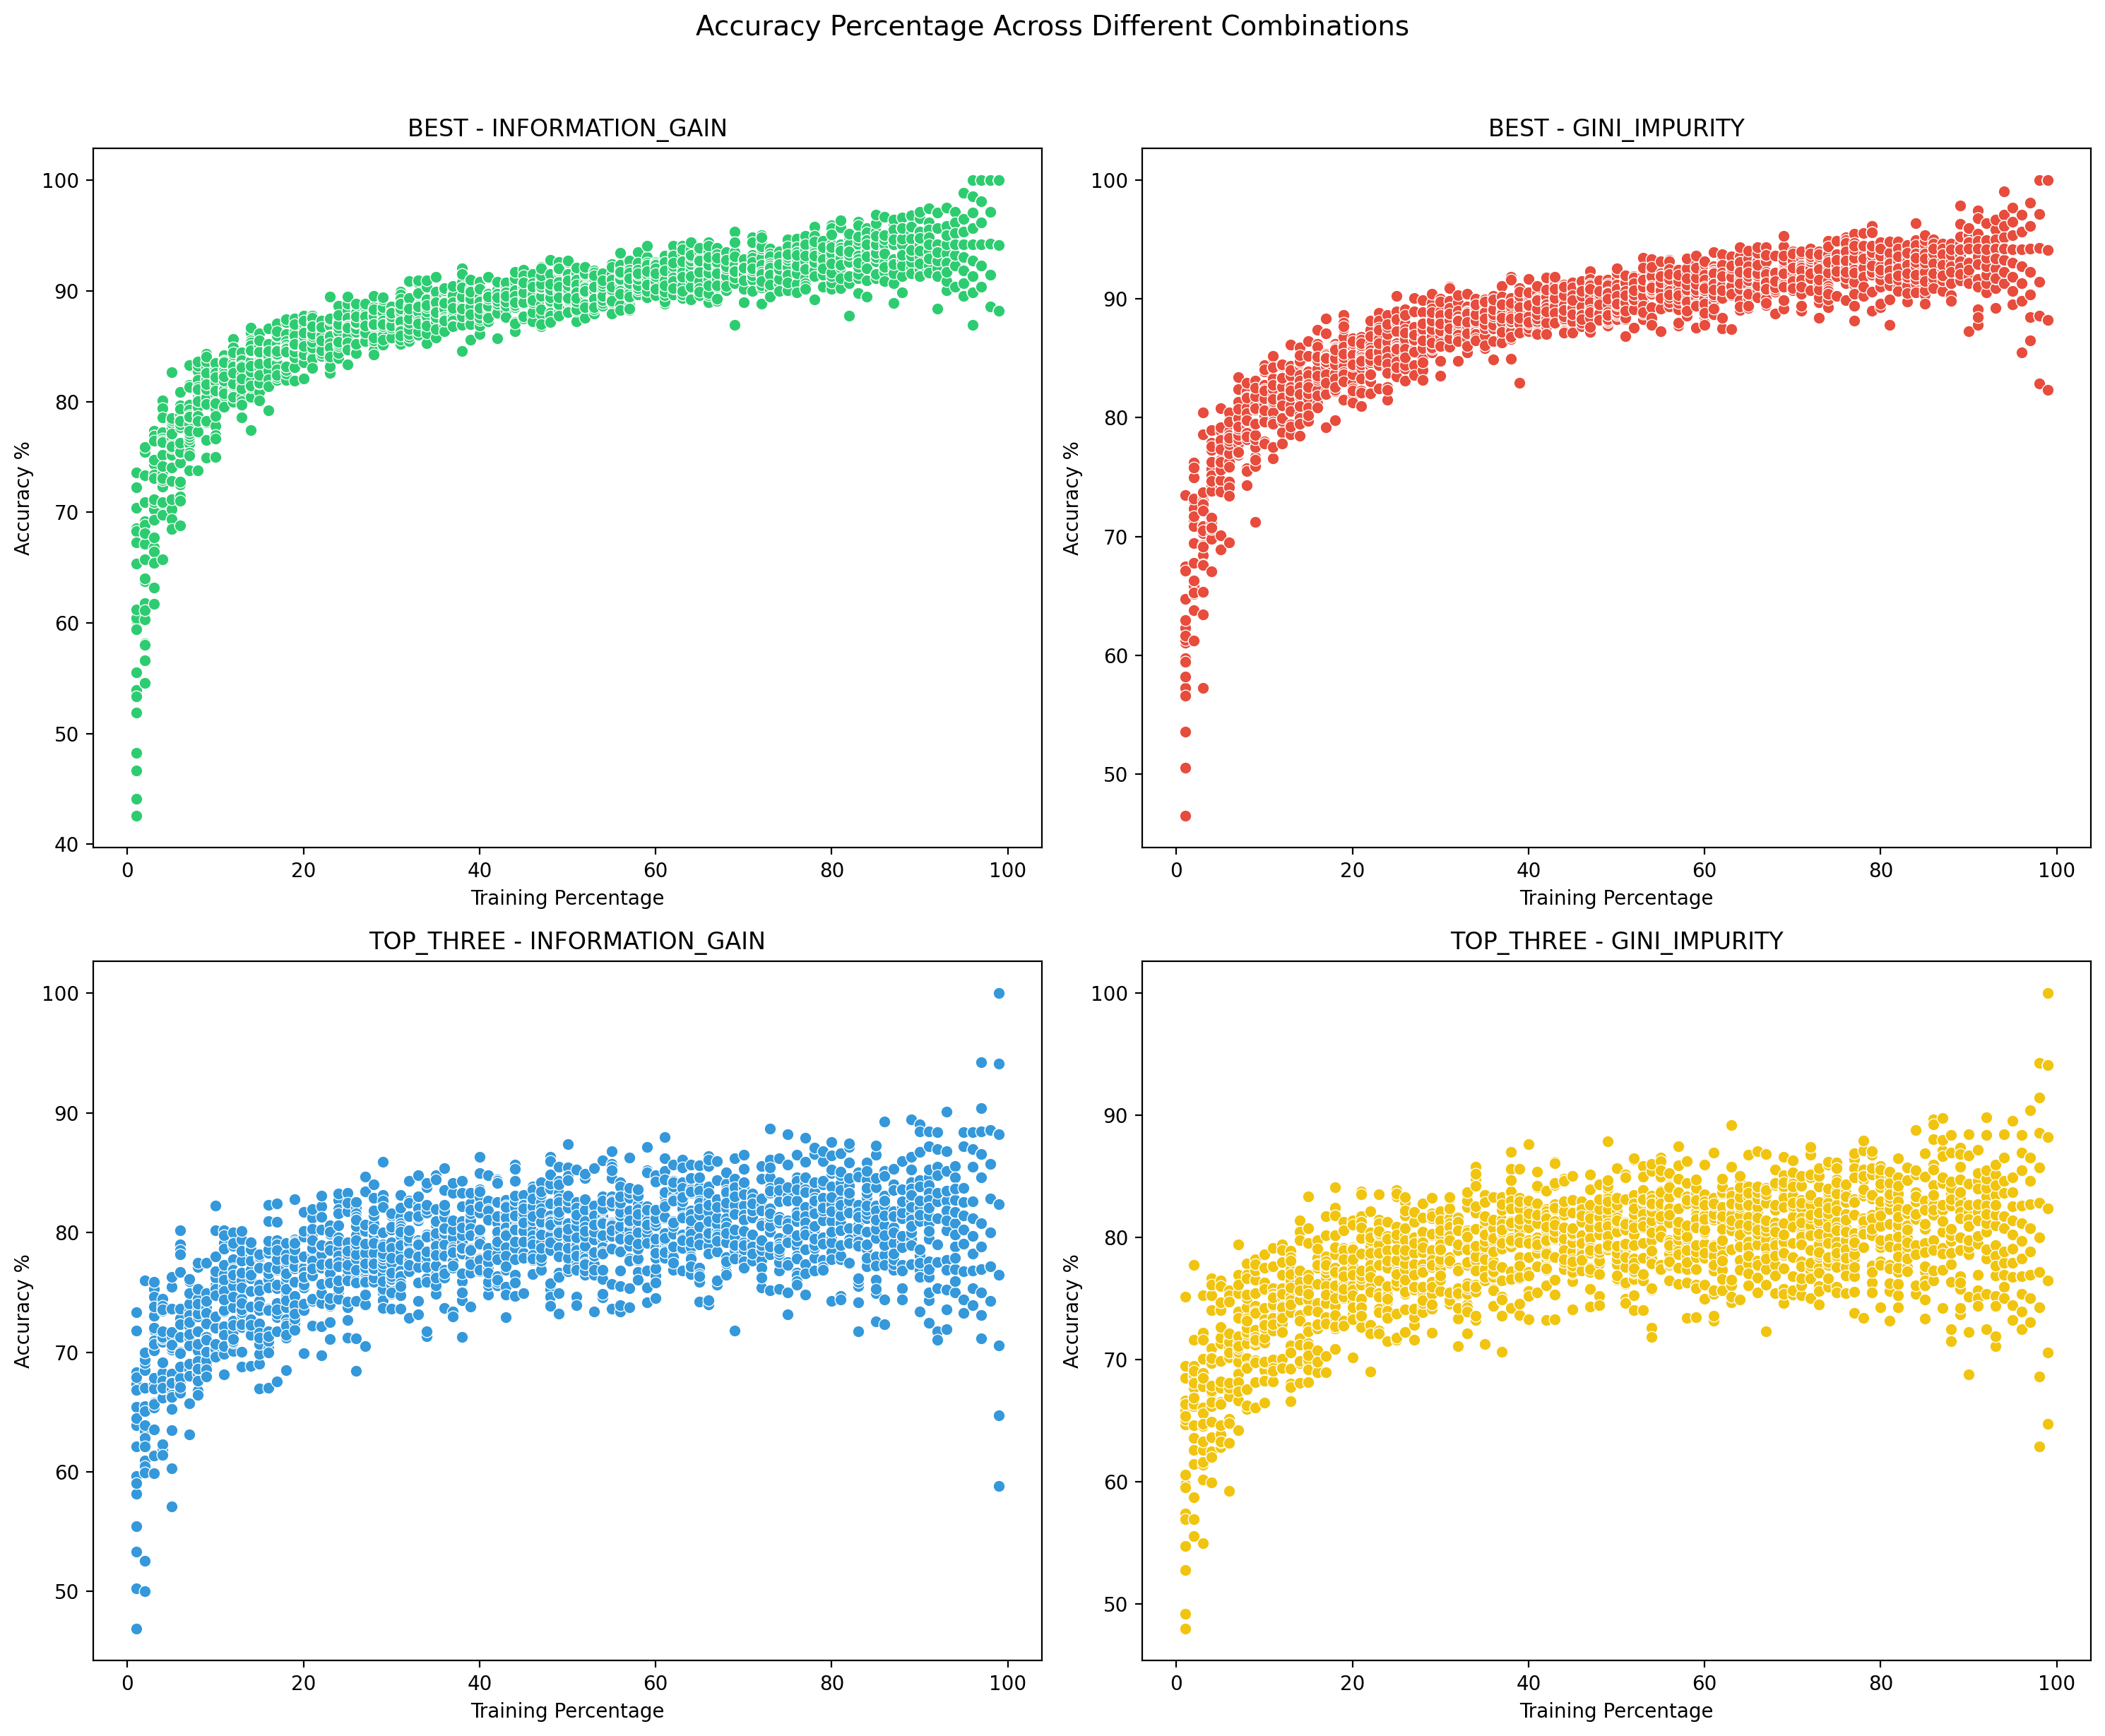
\includegraphics[width=\textwidth]{plots/training_accuracy_combined.png}
    \caption{Accuracy percentage trends across different strategy-metric combinations showing how accuracy varies with training data percentage.}
    \label{fig:training-accuracy}
\end{figure}

The above scatter plots demonstrate how the training accuracy varies over the training percentage. As we increase the percentage of train set in the split from 1\% towards 99\%, the accuracy first increase very fast and then grows slower. Moreover, the accuracy grows much faster and more consistently in the case of choosing the best attribute.

\newpage

\begin{figure}[H]
    \centering
    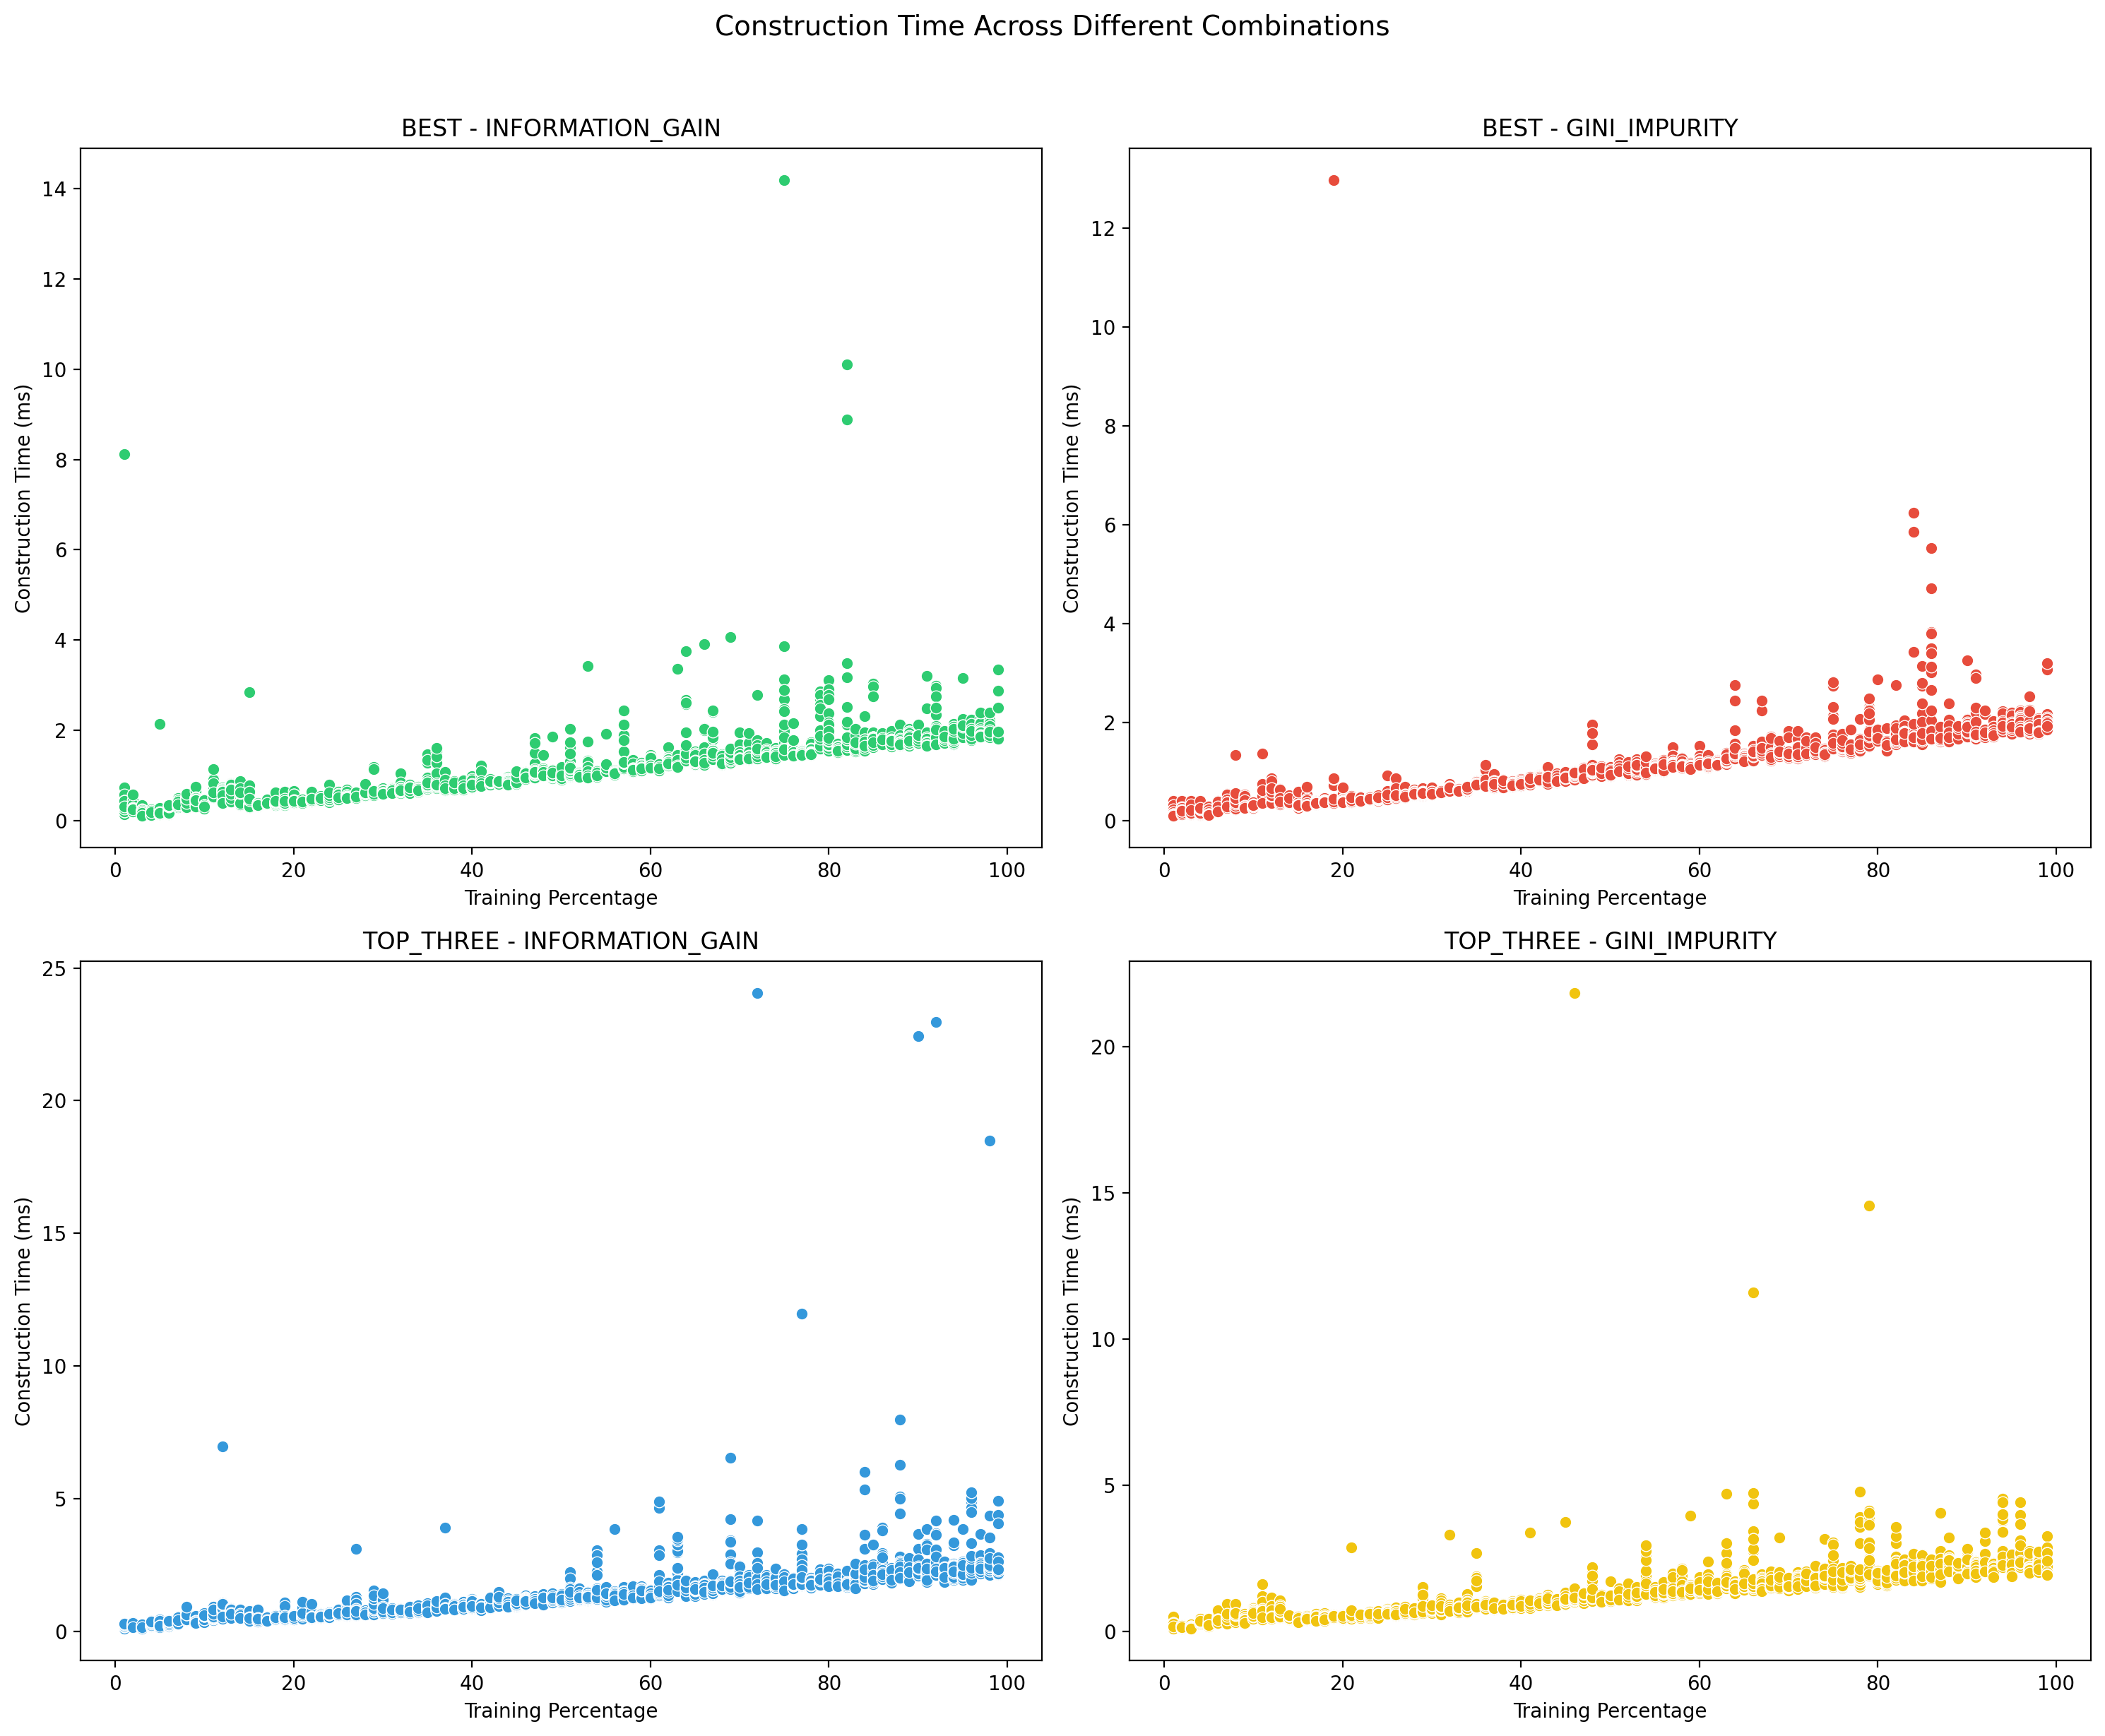
\includegraphics[width=\textwidth]{plots/training_time_combined.png}
    \caption{Construction time comparison across different strategy-metric combinations showing how build time varies with training data size.}
    \label{fig:training-time}
\end{figure}

The above scatter plots demonstrate how the construction time varies over the training percentage. As we increase the percentage of train set in the split from 1\% towards 99\%, the time almost always increases linearly, with some outliers. Naturally, the strategy and metrics do not much affect the construction time.

\newpage

\begin{figure}[H]
    \centering
    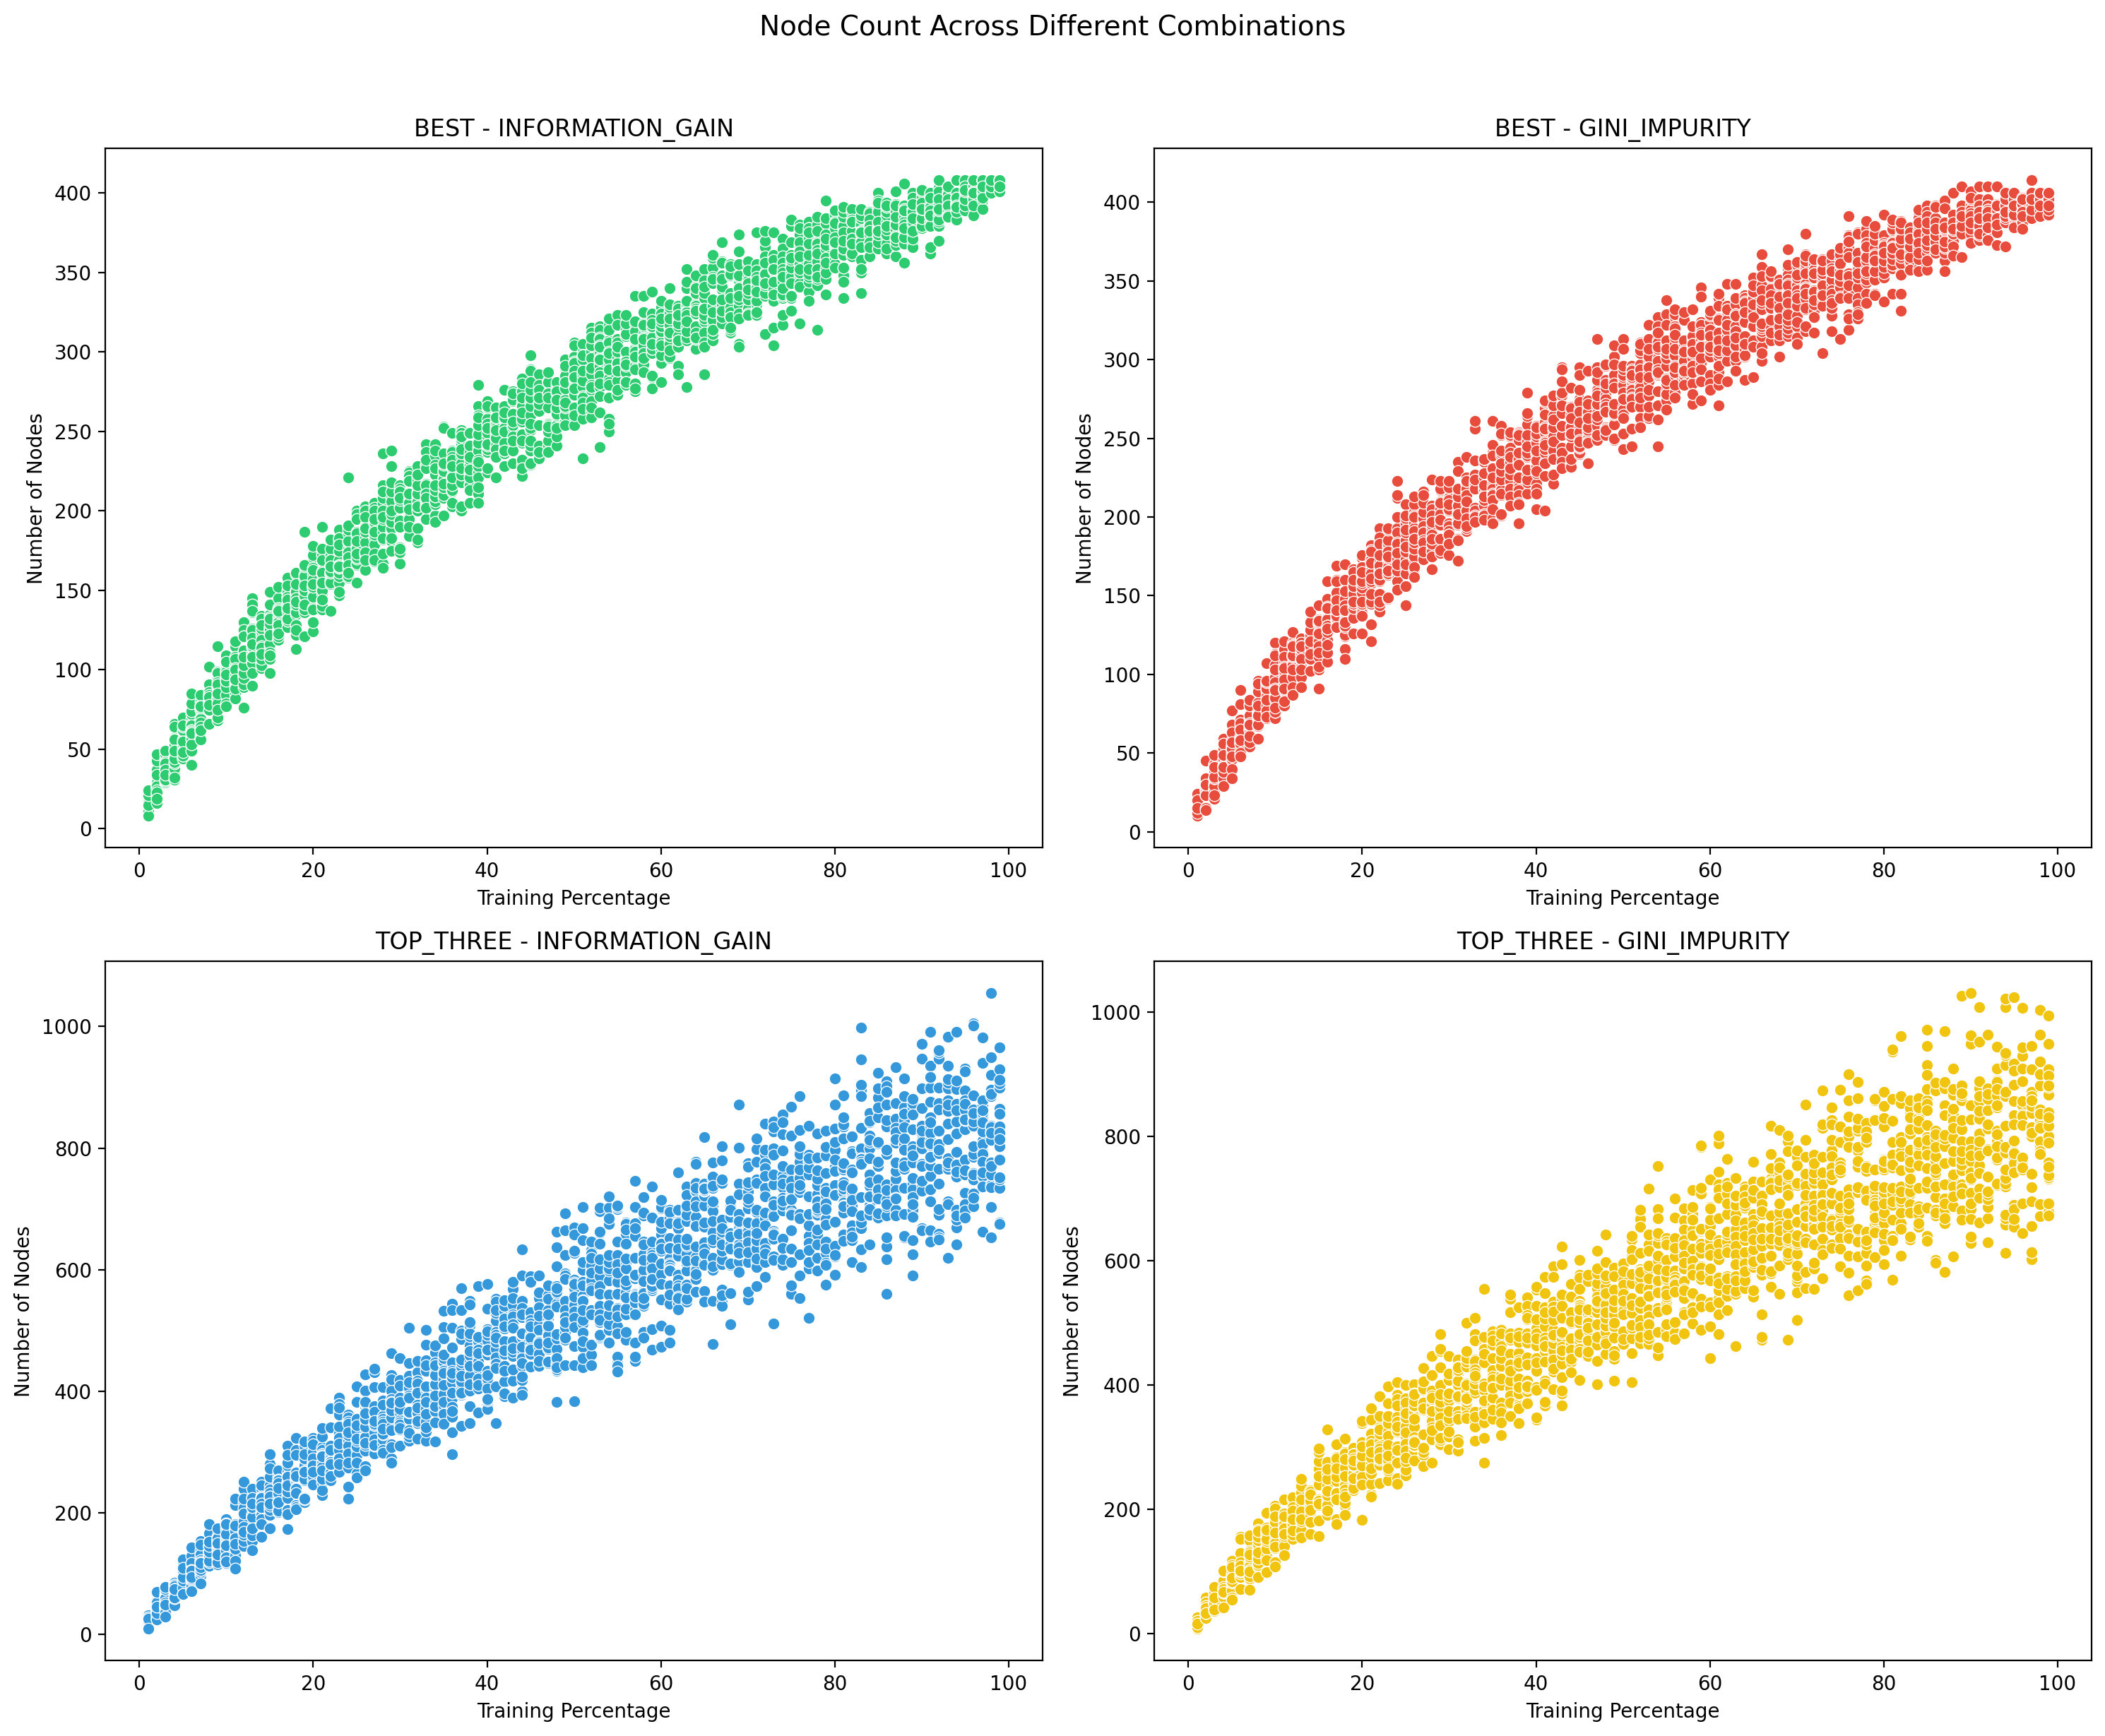
\includegraphics[width=\textwidth]{plots/training_nodes_combined.png}
    \caption{Node count comparison across different strategy-metric combinations showing how tree size varies with training data percentage.}
    \label{fig:training-nodes}
\end{figure}

The above scatter plots demonstrate how the tree node count varies over the training percentage. As we increase the percentage of train set in the split from 1\% towards 99\%, the node count consistently increases. In case of choosing top three and using Gini Impurity, the growth pattern appeared much more scattered.

\end{document}
